\subsection{Wall lamp}
\paragraph{}
In this example, a wall lamp illustrated in Fig.~\ref{oct_ex:lamp_geo_bc} with gravity only is considered.
The material properties are:  Young’s modulus $E = \SI{20}{\newton \per \meter^2}$, Poisson’s ratio $\nu = 0.3$ and density $\rho = \SI{2}{\newton \per \meter^3}$.
\begin{figure}
    \centering
    \scalebox{0.5}{
        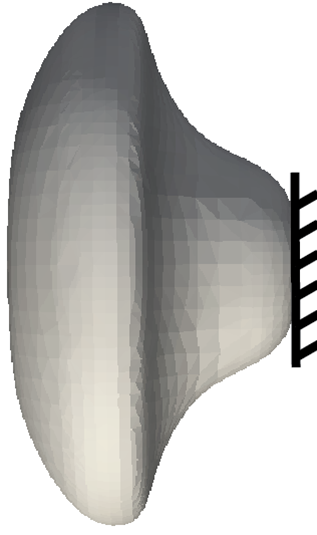
\includegraphics{octree/ex_images/lamp_geo_bc.png}
    }
    \caption[Boundary condition of the wall lamp]{Boundary condition of the wall lamp}
    \label{oct_ex:lamp_geo_bc}
\end{figure}

\paragraph{}
The geometric model is extracted from the AutoCAD as illustrated in Fig.~\ref{oct_ex:lamp_cad}.
\begin{figure}[!ht]
    \centering
    \scalebox{0.5}{
        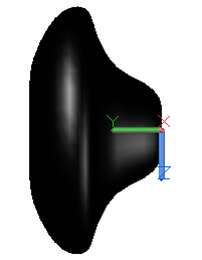
\includegraphics{octree/ex_images/lamp_cad.png}
    }
    \caption[CAD drawing of the wall lamp]{CAD drawing of the wall lamp}
    \label{oct_ex:lamp_cad}
\end{figure}
%
The background mesh before cutting is shown in Fig.~\ref{oct_ex:lamp_mesh_bg}.
\begin{figure}[!ht]
    \centering
    \begin{subfigure}[b]{0.49\linewidth}
        \centering
        \scalebox{0.65}{
            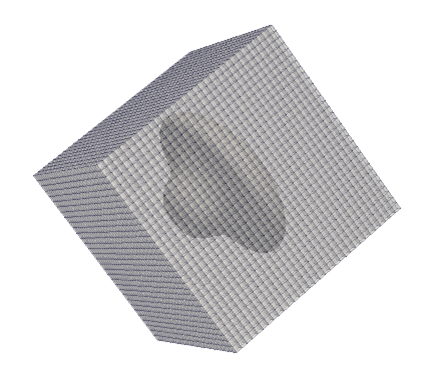
\includegraphics{octree/ex_images/lamp_mesh_bg.png}
        }
    \end{subfigure}
    \begin{subfigure}[b]{0.49\linewidth}
        \centering
        \scalebox{0.65}{
            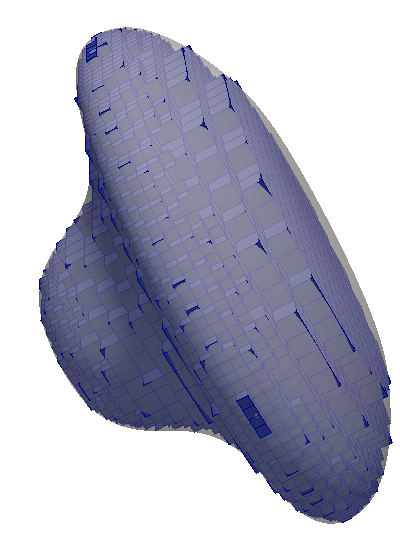
\includegraphics{octree/ex_images/lamp_mesh_bg_2.png}
        }
    \end{subfigure}
    \caption[Background mesh of the wall lamp]{Background mesh of the wall lamp; left: background mesh; right: background mesh around the boundary}.
    \label{oct_ex:lamp_mesh_bg}
\end{figure}
%
The generated mesh are plotted in Fig.~\ref{oct_ex:lamp_mesh}.
\begin{figure}[!ht]
    \centering
    \begin{subfigure}[b]{1\linewidth}
        \centering
        \scalebox{0.75}{
            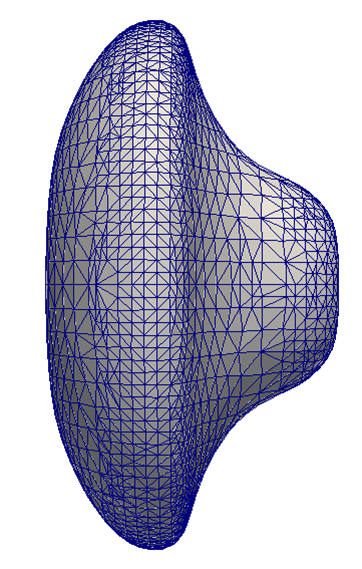
\includegraphics{octree/ex_images/lamp_mesh.png}
        }
    \end{subfigure} \\
    \begin{subfigure}[b]{0.48\linewidth}
        \centering
        \scalebox{0.75}{
            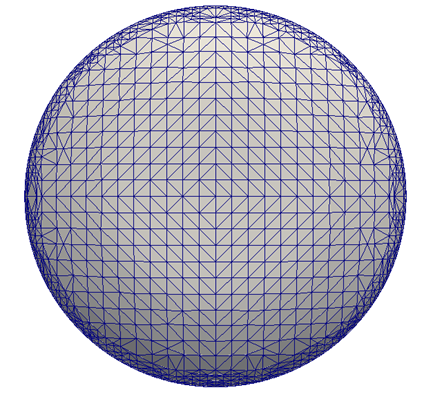
\includegraphics{octree/ex_images/lamp_mesh_front.png}
        }
    \end{subfigure}
    \begin{subfigure}[b]{0.48\linewidth}
        \centering
        \scalebox{0.75}{
            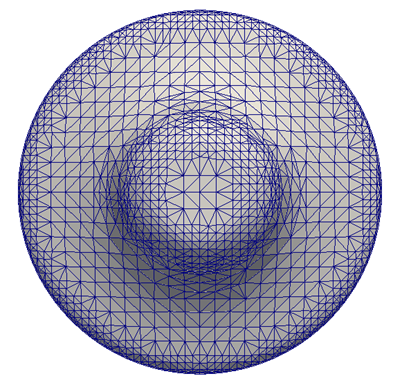
\includegraphics{octree/ex_images/lamp_mesh_back.png}
        }
    \end{subfigure}
    \caption[Mesh of the wall lamp]{Mesh of the wall lamp}
    \label{oct_ex:lamp_mesh}
\end{figure}
%
The displacement is plotted as deformed shape in Fig.~\ref{oct_ex:lamp_deformed_shape}.
\begin{figure}[!ht]
    \centering
    \scalebox{0.5}{
        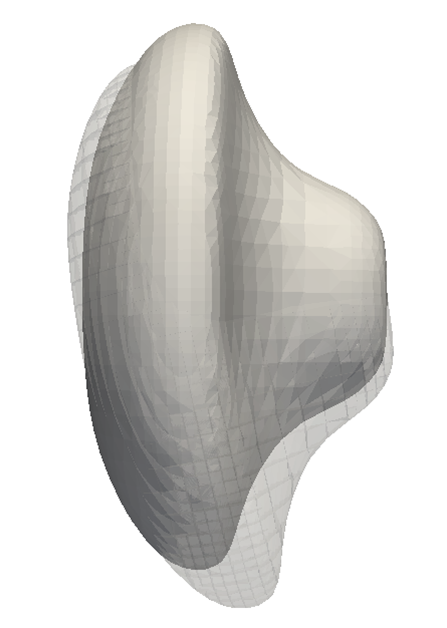
\includegraphics{octree/ex_images/lamp_deformed_shape.png}
    }
    \caption[Deformed shape of the wall lamp]{Deformed shape of the wall lamp}
    \label{oct_ex:lamp_deformed_shape}
\end{figure}
